
\chapter*{Appendix}
\label{chap:TXT-text}
\pagestyle{plain}
%link to url
%authorship
%origin buge grandmother of Kanganu
%distribution of booklet
%
\section*{Background and introduction of the narrative texts}
\label{chap:TXT-text-2}

Two interlinearized narrative texts and their respective translation are
offrered in this appendix. They consist of oral third person traditional folk
tales, recited by Daniel Karija Kanganu. The stories  were passed down to him by
his grand-mother, a woman from Buge (9° 37' 0" North, 1° 54' 0" West, Vagla
land) who married a man from Ducie, so lived most of her adult life there.
They were first recited to me in 2007, at which occasion they were transcribed, 
and then made available as two short books \citep{Kang07b, Kang07a}.  At that
time, the intention was to introduce a Chakali orthography to the schools in
Ducie, Motigu, Katua and Gurumbele. A year later, the transcription of the text
was further improved. 


The two narratives are introduced by English translations. The overall text is
represented with a  five-tier linguistic annotation.  The interlinearized text
comprises four lines of information. The first line (i.e. tx) represents the
object language which receives an impressionistic tone annotation and a unified
orthography. The latter is inspired by the language's description of chapter
\ref{sec:chap-phono} and \ref{sec:gramsketch}. The second line (i.e. mb)
represents the `morpheme-break'-level capturing the units included in the
lexicon. The third line (i.e. ge) contains  the  units' glosses, and the fourth
line (i.e. ps) gives their respective part of speech. Each block of
interlinearized text (i.e. ref) is accompanied of an idiomatic English
rendition (i.e. ft). 




\cleardoublepage

%%%%%%%%%%%%%%%%%%%%%%%%%%%


%\pagebreak
\section*{Text 1}
\label{chap:TXT-text-1}

\vspace*{30pt}
\begin{center}
 {\Large beŋ tʃelle}\\
{\large The law breaker}
\end{center}


Once upon a time there was a landlord who let it be known that no one should
mention the number eight. If anyone should refuse and say the number, they would
be put to death. Spider set up his farm by a main road. Everyone that came along
the road asked Spider what he was doing there. Spider would reply that his
family  was now becoming bigger and if he did not have a large farm, he would
not have enough to feed his many children. He made many yam mounds at the farm.
One day, Buffalo came to his farm. Spider asked Buffalo to count the yam mounds
for him, because when he tried to count them himself he became confused. Buffalo
started counting,  “One, two, three, four, five, six, seven, eight, nine, ten.”
Spider told Buffalo that the landlord said anyone who said the number eight
should be taken to him. Buffalo agreed with Spider,  “Kill me so that your family
can eat.” Spider killed Buffalo and he and his family lived on Buffalo’s meat.
One day Monkey also went to Spider’s farm to greet him. Spider said, “Monkey,
come and drink water.” Monkey quickly went and sat on the eighth yam mound.
Then Spider asked Monkey,  “Count the yam mounds for me.” Monkey started
counting,  “One, two, three, four, five, six, seven, the one I’m sitting on,
nine, ten.” Spider said he did not count well, so he should repeat it. Monkey
repeated,  “One, two, three, four, five, six, seven, the one I’m sitting on,
nine, ten.” Then Spider became furious, boiling as he said to Monkey,  “Can’t
you count one, two, three, four, five, six, seven, eight, nine, ten?” Monkey
said, “The landlord said no one should call the number eight and you did it,
so let’s go to the landlord and tell him that you called the number eight.” 
They
both went to the landlord and, yes, Spider had indeed broken the law.  Monkey
swallowed him, but Spider got stuck in Monkey’s throat. That’s why the monkey
sounds like “angumm, angumm, angumm”. That marks the end of our story.

%FIX They both went to the landlord and it was Spider who had broken the law

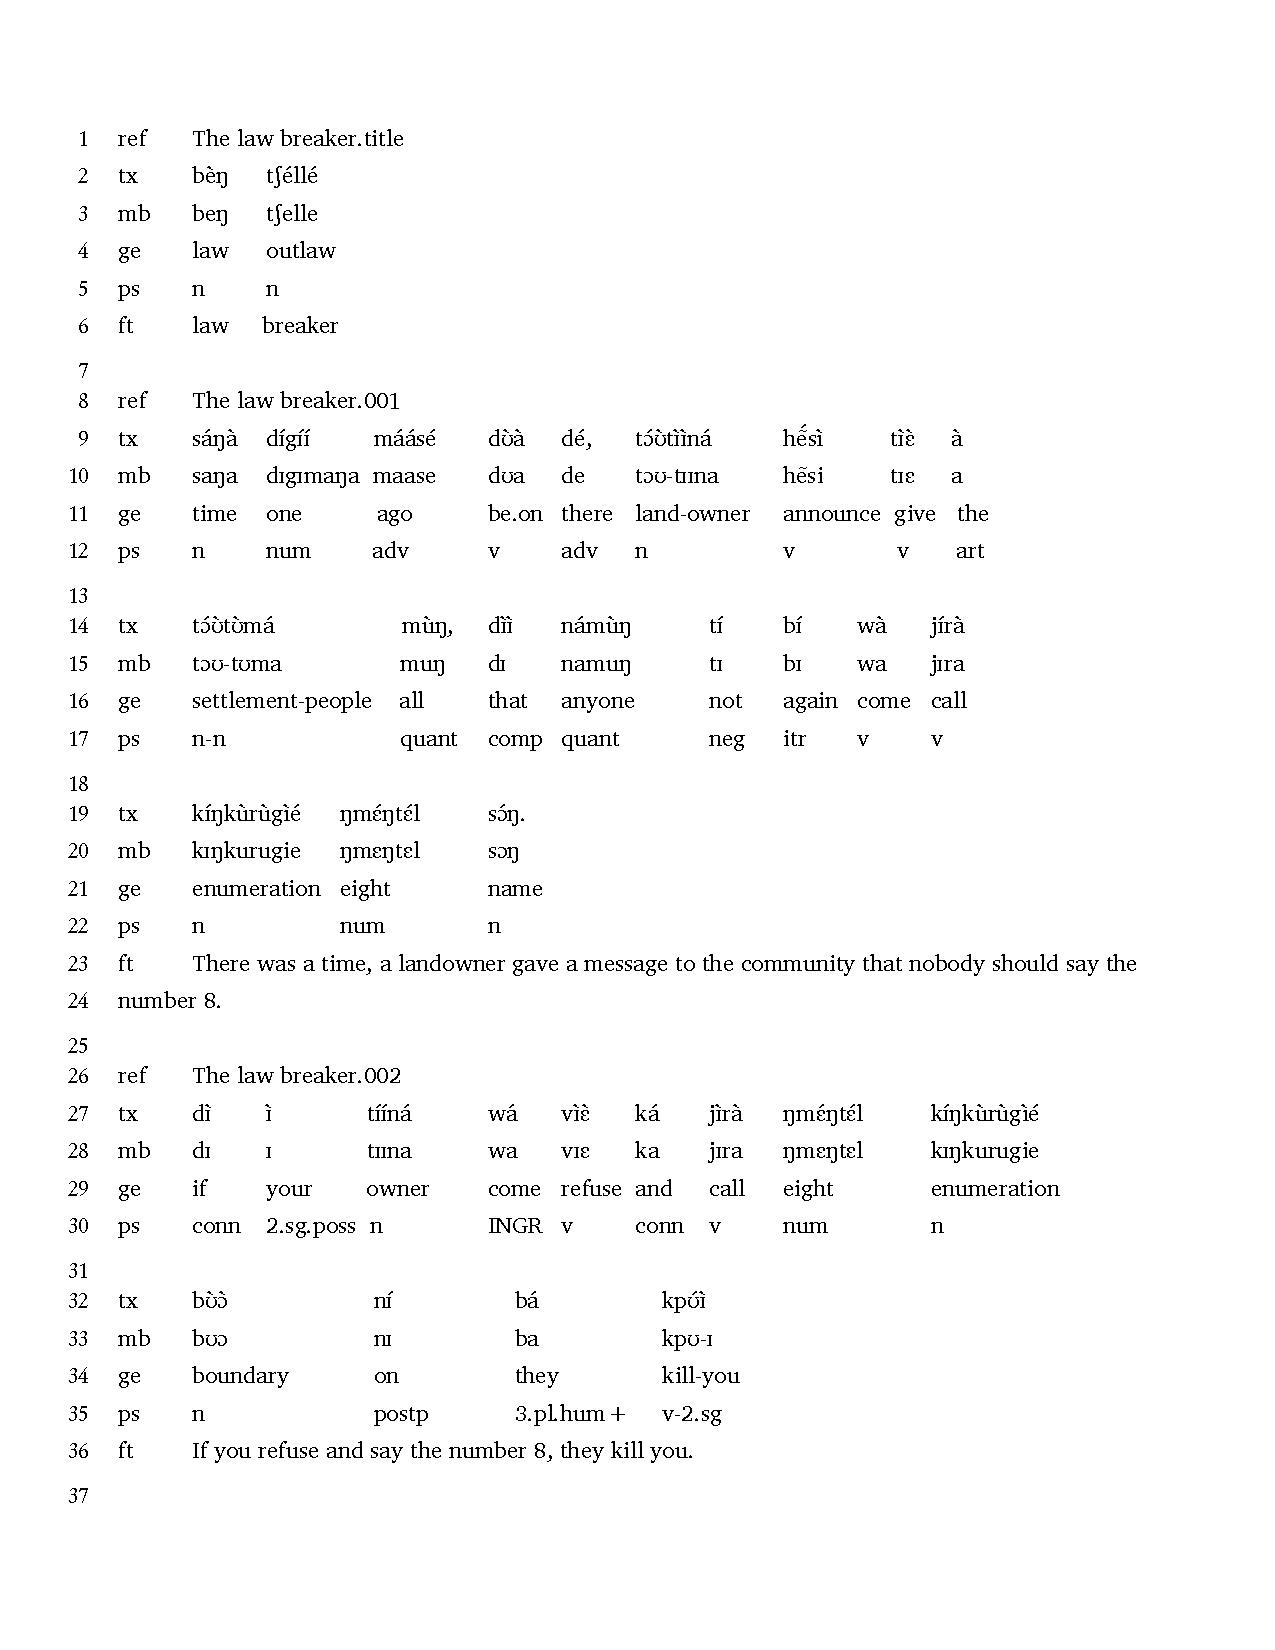
\includepdf[pages=1-9, scale=.8,
pagecommand={\thispagestyle{plain}}]{Graphic/Pictures/law-inter.pdf}

%%%%%%%%%%%%%%%%%%%%%%%%%%%%%%%%%%%%%%%%%%%%%%%%%
%%%%%%%%%%%%%%%%%%%%%%%%%%%%%%%%%%%%%%%%%%%%%%%%%%%


\cleardoublepage


\section*{Text 2}
\label{chap:TXT-text-2}

\vspace*{30pt}
\begin{center}
 {\Large bɪpɔlɪɪ naŋzɪmatɪɪna}\\
 {\large The clever boy}\\
\end{center}


 Once upon a time a chief had a daughter. One day he said that whoever
wanted to marry his daughter should go to his farm and work for a day before
he would sanction the marriage. At the chief’s farm there were many tsetse
flies. The chief required that the person doing the work should not kill any of
the tsetse flies landing on him. If he did so, he would not be allowed to marry
the girl. One young man told the chief that he would weed the farm and
take the daughter. The following day the young man brought his hoe and
the chief asked his daughter to accompany the man to the farm to witness the
feat. The young man was weeding while the young girl was
watching him to ensure that he did not kill or even hit a single tsetse fly.
The tsetse flies were biting the man but he was not allowed to kill any. The
young
man asked the girl, “When your father kills game, which part does he give
you?” The young girl said, “When my father kills game, he gives me the
head.” The young man stood straight and said, “Is that true? When your
father kills game, have you never seen the leg, the hand, the flank, the neck,
or any other parts of the animal apart from the head?” The chief’s daughter
answered “Yes”. In the process of asking and demonstrating which body parts, the
young man
was hitting his leg, arm, side and every part of his body. He killed all the
tsetse flies  without the girl noticing and had a chance to weed the farm.
When they went home, the girl told her father the young man had finished weeding
without killing or driving away a single tsetse fly. The chief said,
“Is that true? So he is your husband, you will marry him and you will be
together until the end of your life.”  The girl married the young man and
they had children. Sometimes, the woman would insult the man. When
misunderstandings arose between them, she would tell him that he was foolish
and stupid. The man said, “Do you know the sort of knowledge I used to
weed your father’s farm before I had you as a wife? Do you remember the
time I was weeding your father’s farm while asking you about the animal parts
he used to give you? You said, `My father gives me the head.' When I was
demonstrating by touching my leg,  hand, side, neck and every 
part of my body,  I was actually chasing the tsetse flies away. I used my
cunning to drive the tsetse flies away and weed the farm and take you as a
wife. Yet you insult me, calling me a fool.” The girl said, “So I will go and
tell my father how you cheated, and  killed the tsetse
flies while weeding, so you could take me as a wife.”  The man replied, “You
should be
patient
until tomorrow. You cannot wake up a chief.” She agreed and slept. That
very night the husband smashed some dawadawa and put some of it on the
woman’s bed. He also pulled down her underwear a bit and put some around
her anus.
 Then, he covered her. Early in the morning, the man woke  his wife from sleep.
The woman awoke and thought there was feces in her bed and even around her anus.
The woman sat quietly and did not
know what to do. The man asked her, “Are you the one who defecated 
in bed?” The woman was ashamed and cried. The man said, “Don’t cry, if
you don't tell your father that I drove the tsetse flies away when I was weeding,
I
will not tell your father that you relieved yourself in bed.” Then the wife
said,
“No, I won’t say anything to my father again.” This marks the end of our
story.




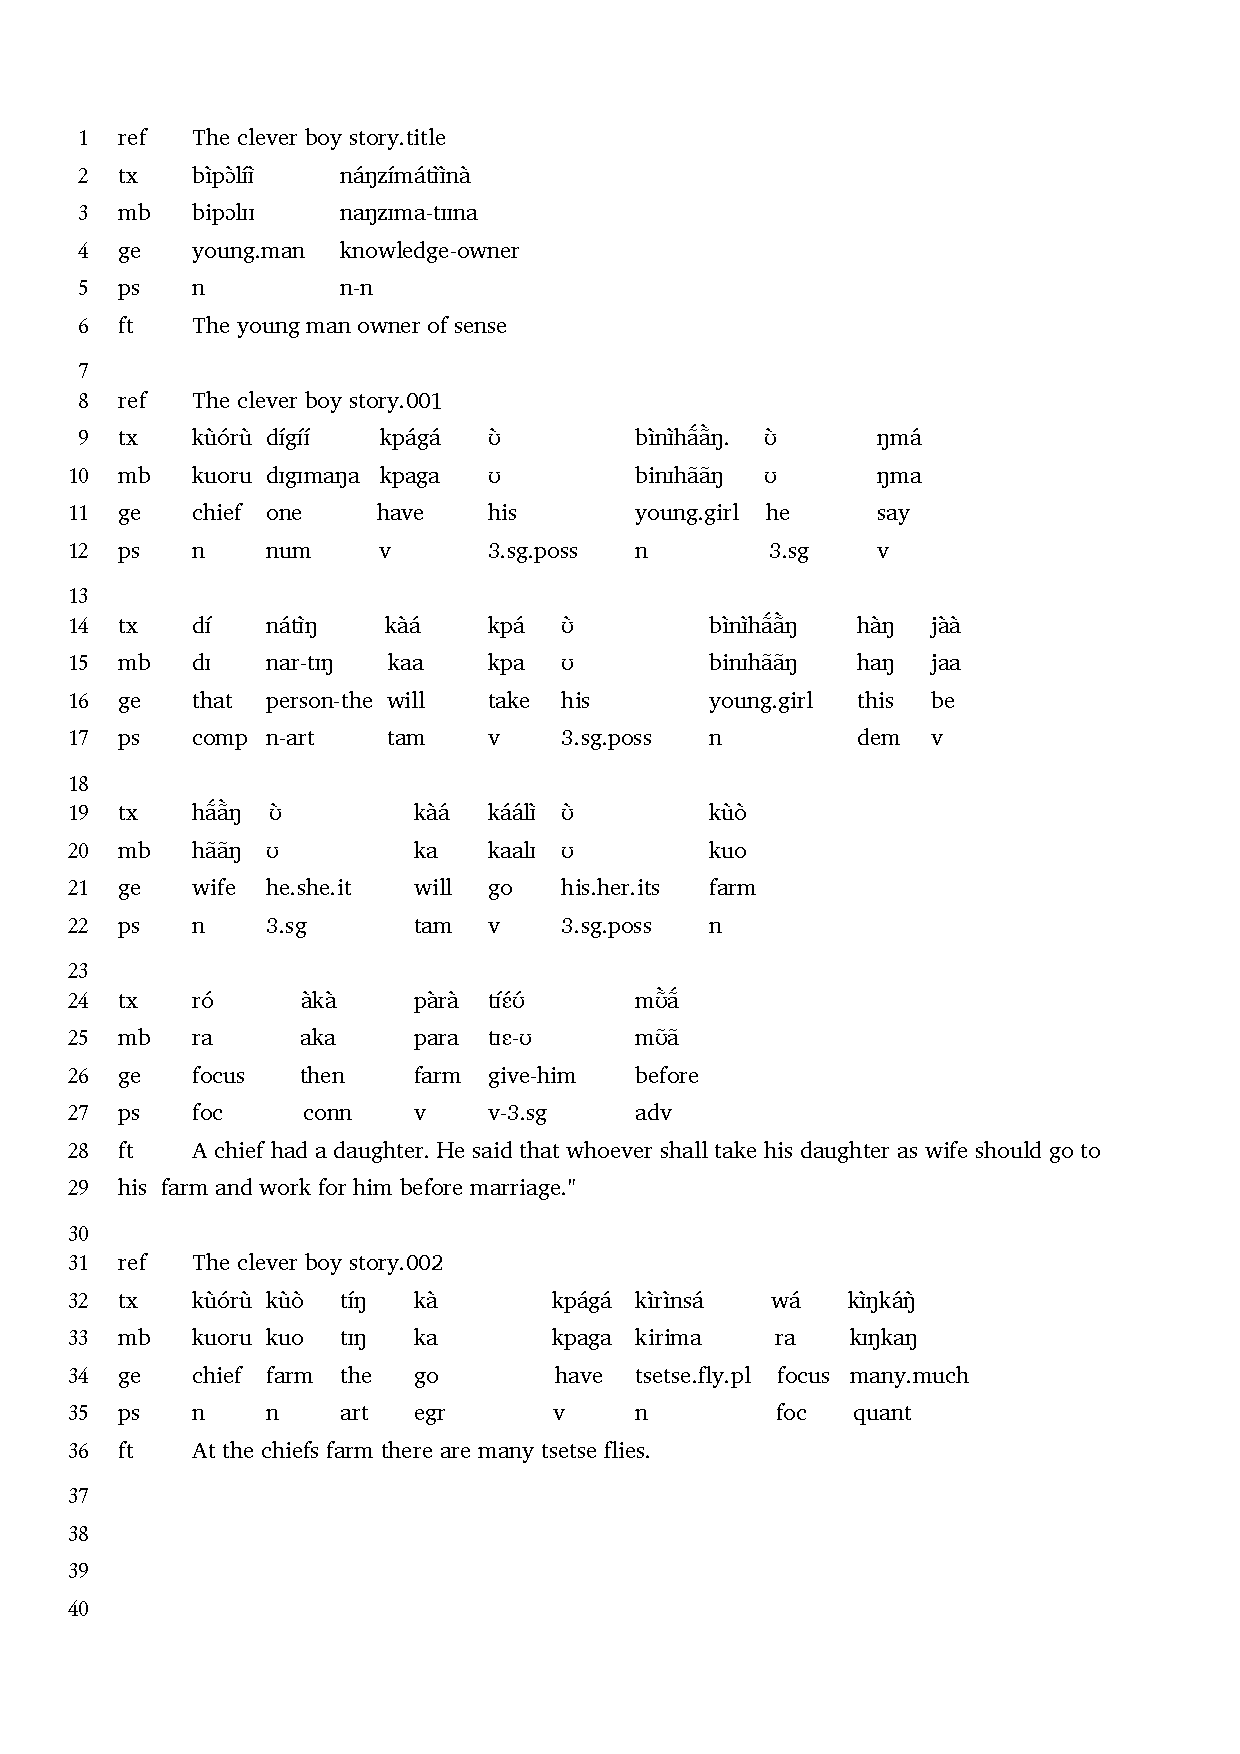
\includepdf[pages=1-16, scale=.8,
pagecommand={\thispagestyle{plain}}]{Graphic/Pictures/clever-inter.pdf}








